\documentclass[journal,12pt,twocolumn]{IEEEtran}
%
\usepackage{setspace}
\usepackage{gensymb}
%\doublespacing
\singlespacing

%\usepackage{graphicx}
%\usepackage{amssymb}
%\usepackage{relsize}
\usepackage[cmex10]{amsmath}
%\usepackage{amsthm}
%\interdisplaylinepenalty=2500
%\savesymbol{iint}
%\usepackage{txfonts}
%\restoresymbol{TXF}{iint}
%\usepackage{wasysym}
\usepackage{amsthm}
%\usepackage{iithtlc}
\usepackage{mathrsfs}
\usepackage{txfonts}
\usepackage{stfloats}
\usepackage{bm}
\usepackage{cite}
\usepackage{cases}
\usepackage{subfig}
%\usepackage{xtab}
\usepackage{longtable}
\usepackage{multirow}
%\usepackage{algorithm}
%\usepackage{algpseudocode}
\usepackage{enumitem}
\usepackage{mathtools}
\usepackage{tikz}
\usepackage[american]{circuitikz}
\usepackage{verbatim}
\usepackage{tfrupee}
\usepackage[breaklinks=true]{hyperref}
%\usepackage{stmaryrd}
\usepackage{tkz-euclide} % loads  TikZ and tkz-base
%\usetkzobj{all}
\usetikzlibrary{decorations.markings}
\usetikzlibrary{shapes.geometric}
\newif\iflabrev
\usepackage{listings}
    \usepackage{color}                                            %%
    \usepackage{array}                                            %%
    \usepackage{longtable}                                        %%
    \usepackage{calc}                                             %%
    \usepackage{multirow}                                         %%
    \usepackage{hhline}                                           %%
    \usepackage{ifthen}                                           %%
  %optionally (for landscape tables embedded in another document): %%
    \usepackage{lscape}     
\usepackage{multicol}
\usepackage{chngcntr}
%\usepackage{enumerate}

%\usepackage{wasysym}
%\newcounter{MYtempeqncnt}
\DeclareMathOperator*{\Res}{Res}
%\renewcommand{\baselinestretch}{2}
\renewcommand\thesection{\arabic{section}}
\renewcommand\thesubsection{\thesection.\arabic{subsection}}
\renewcommand\thesubsubsection{\thesubsection.\arabic{subsubsection}}

\renewcommand\thesectiondis{\arabic{section}}
\renewcommand\thesubsectiondis{\thesectiondis.\arabic{subsection}}
\renewcommand\thesubsubsectiondis{\thesubsectiondis.\arabic{subsubsection}}

% correct bad hyphenation here
\hyphenation{op-tical net-works semi-conduc-tor}
\def\inputGnumericTable{}                                 %%

\lstset{
%language=C,
frame=single, 
breaklines=true,
columns=fullflexible
}
%\lstset{
%language=tex,
%frame=single, 
%breaklines=true
%}

\begin{document}
%


\newtheorem{theorem}{Theorem}[section]
\newtheorem{problem}{Problem}
\newtheorem{proposition}{Proposition}[section]
\newtheorem{lemma}{Lemma}[section]
\newtheorem{corollary}[theorem]{Corollary}
\newtheorem{example}{Example}[section]
\newtheorem{definition}[problem]{Definition}
%\newtheorem{thm}{Theorem}[section] 
%\newtheorem{defn}[thm]{Definition}
%\newtheorem{algorithm}{Algorithm}[section]
%\newtheorem{cor}{Corollary}
\newcommand{\BEQA}{\begin{eqnarray}}
\newcommand{\EEQA}{\end{eqnarray}}
\newcommand{\define}{\stackrel{\triangle}{=}}
\bibliographystyle{IEEEtran}
%\bibliographystyle{ieeetr}
\providecommand{\mbf}{\mathbf}
\providecommand{\pr}[1]{\ensuremath{\Pr\left(#1\right)}}
\providecommand{\qfunc}[1]{\ensuremath{Q\left(#1\right)}}
\providecommand{\sbrak}[1]{\ensuremath{{}\left[#1\right]}}
\providecommand{\lsbrak}[1]{\ensuremath{{}\left[#1\right.}}
\providecommand{\rsbrak}[1]{\ensuremath{{}\left.#1\right]}}
\providecommand{\brak}[1]{\ensuremath{\left(#1\right)}}
\providecommand{\lbrak}[1]{\ensuremath{\left(#1\right.}}
\providecommand{\rbrak}[1]{\ensuremath{\left.#1\right)}}
\providecommand{\cbrak}[1]{\ensuremath{\left\{#1\right\}}}
\providecommand{\lcbrak}[1]{\ensuremath{\left\{#1\right.}}
\providecommand{\rcbrak}[1]{\ensuremath{\left.#1\right\}}}
\theoremstyle{remark}
\newtheorem{rem}{Remark}
\newcommand{\sgn}{\mathop{\mathrm{sgn}}}
\providecommand{\abs}[1]{\left\vert#1\right\vert}
\providecommand{\res}[1]{\Res\displaylimits_{#1}} 
\providecommand{\norm}[1]{\left\lVert#1\right\rVert}
%\providecommand{\norm}[1]{\lVert#1\rVert}
\providecommand{\mtx}[1]{\mathbf{#1}}
\providecommand{\mean}[1]{E\left[ #1 \right]}
\providecommand{\fourier}{\overset{\mathcal{F}}{ \rightleftharpoons}}
%\providecommand{\hilbert}{\overset{\mathcal{H}}{ \rightleftharpoons}}
\providecommand{\system}{\overset{\mathcal{H}}{ \longleftrightarrow}}
	%\newcommand{\solution}[2]{\textbf{Solution:}{#1}}
\newcommand{\solution}{\noindent \textbf{Solution: }}
\newcommand{\cosec}{\,\text{cosec}\,}
\providecommand{\dec}[2]{\ensuremath{\overset{#1}{\underset{#2}{\gtrless}}}}
\newcommand{\myvec}[1]{\ensuremath{\begin{pmatrix}#1\end{pmatrix}}}
\newcommand{\mydet}[1]{\ensuremath{\begin{vmatrix}#1\end{vmatrix}}}
%\numberwithin{equation}{section}
\numberwithin{equation}{subsection}
%\numberwithin{problem}{section}
%\numberwithin{definition}{section}
\makeatletter
\@addtoreset{figure}{problem}
\makeatother
\let\StandardTheFigure\thefigure
\let\vec\mathbf
%\renewcommand{\thefigure}{\theproblem.\arabic{figure}}
\renewcommand{\thefigure}{\theproblem}
%\setlist[enumerate,1]{before=\renewcommand\theequation{\theenumi.\arabic{equation}}
%\counterwithin{equation}{enumi}
%\renewcommand{\theequation}{\arabic{subsection}.\arabic{equation}}
\def\putbox#1#2#3{\makebox[0in][l]{\makebox[#1][l]{}\raisebox{\baselineskip}[0in][0in]{\raisebox{#2}[0in][0in]{#3}}}}
     \def\rightbox#1{\makebox[0in][r]{#1}}
     \def\centbox#1{\makebox[0in]{#1}}
     \def\topbox#1{\raisebox{-\baselineskip}[0in][0in]{#1}}
     \def\midbox#1{\raisebox{-0.5\baselineskip}[0in][0in]{#1}}
\vspace{3cm}
\title{
%	\logo{
Wein-bridge oscillator
%	}
}
\author{ Vedala Sai Ashok$^{*}$% <-this % stops a space
	\thanks{*The author is with the Department
		of Electrical Engineering, Indian Institute of Technology, Hyderabad
		502285 India. All content in this manual is released under GNU GPL.  Free and open source.}
	
}	
%\title{
%	\logo{Matrix Analysis through Octave}{\begin{center}\includegraphics[scale=.24]{tlc}\end{center}}{}{HAMDSP}
%}
% paper title
% can use linebreaks \\ within to get better formatting as desired
%\title{Matrix Analysis through Octave}
%
%
% author names and IEEE memberships
% note positions of commas and nonbreaking spaces ( ~ ) LaTeX will not break
% a structure at a ~ so this keeps an author's name from being broken across
% two lines.
% use \thanks{} to gain access to the first footnote area
% a separate \thanks must be used for each paragraph as LaTeX2e's \thanks
% was not built to handle multiple paragraphs
%
%\author{<-this % stops a space
%\thanks{}}
%}
% note the % following the last \IEEEmembership and also \thanks - 
% these prevent an unwanted space from occurring between the last author name
% and the end of the author line. i.e., if you had this:
% 
% \author{....lastname \thanks{...} \thanks{...} }
%                     ^------------^------------^----Do not want these spaces!
%
% a space would be appended to the last name and could cause every name on that
% line to be shifted left slightly. This is one of those "LaTeX things". For
% instance, "\textbf{A} \textbf{B}" will typeset as "A B" not "AB". To get
% "AB" then you have to do: "\textbf{A}\textbf{B}"
% \thanks is no different in this regard, so shield the last } of each \thanks
% that ends a line with a % and do not let a space in before the next \thanks.
% Spaces after \IEEEmembership other than the last one are OK (and needed) as
% you are supposed to have spaces between the names. For what it is worth,
% this is a minor point as most people would not even notice if the said evil
% space somehow managed to creep in.
% The paper headers
%\markboth{Journal of \LaTeX\ Class Files,~Vol.~6, No.~1, January~2007}%
%{Shell \MakeLowercase{\textit{et al.}}: Bare Demo of IEEEtran.cls for Journals}
% The only time the second header will appear is for the odd numbered pages
% after the title page when using the twoside option.
% 
% *** Note that you probably will NOT want to include the author's ***
% *** name in the headers of peer review papers.                   ***
% You can use \ifCLASSOPTIONpeerreview for conditional compilation here if
% you desire.
% If you want to put a publisher's ID mark on the page you can do it like
% this:
%\IEEEpubid{0000--0000/00\$00.00~\copyright~2007 IEEE}
% Remember, if you use this you must call \IEEEpubidadjcol in the second
% column for its text to clear the IEEEpubid mark.
% make the title area
\maketitle
%\newpage
%\tableofcontents
\bigskip
\renewcommand{\thefigure}{\theenumi}
\renewcommand{\thetable}{\theenumi}
%\renewcommand{\theequation}{\theenumi}
%\begin{abstract}
%%\boldmath
%In this letter, an algorithm for evaluating the exact analytical bit error rate  (BER)  for the piecewise linear (PL) combiner for  multiple relays is presented. Previous results were available only for upto three relays. The algorithm is unique in the sense that  the actual mathematical expressions, that are prohibitively large, need not be explicitly obtained. The diversity gain due to multiple relays is shown through plots of the analytical BER, well supported by simulations. 
%
%\end{abstract}
% IEEEtran.cls defaults to using nonbold math in the Abstract.
% This preserves the distinction between vectors and scalars. However,
% if the journal you are submitting to favors bold math in the abstract,
% then you can use LaTeX's standard command \boldmath at the very start
% of the abstract to achieve this. Many IEEE journals frown on math
% in the abstract anyway.
% Note that keywords are not normally used for peerreview papers.
%\begin{IEEEkeywords}
%Cooperative diversity, decode and forward, piecewise linear
%\end{IEEEkeywords}
% For peer review papers, you can put extra information on the cover
% page as needed:
% \ifCLASSOPTIONpeerreview
% \begin{center} \bfseries EDICS Category: 3-BBND \end{center}
% \fi
%
% For peerreview papers, this IEEEtran command inserts a page break and
% creates the second title. It will be ignored for other modes.
%\IEEEpeerreviewmaketitle
%\begin{abstract}
%The objective of this manual is to introduce control system design at an elementary level.
%\end{abstract}
%\section{Feedback Circuits}
Redesign the circuit of Fig. \ref{fig:ee18btech11049_fig1} for operation at 10KHz using same values of resistance. If at 10KHz the op amp provides an excess phase shift (lag) of 5.7\degree , what will be the frequency of oscillation? Assume the phase shift introduced by the op amp remains constant for frequencies around 10KHz.)To restore operation to 10KHz, what change must be made in the shunt resistor of the wien bridge? Also, to what value must $R_{2}/R_{1}$ be changed ?
\begin{figure}[!ht]
	\begin{center}
		\resizebox{\columnwidth}{!}{\begin{circuitikz}[scale = 1]
\draw
(0,0) to[empty diode] (4,0) -- (4,1.5)
    to[R, *-*,l_ = $10k\Omega$] (0,1.5) -- (0,0)
(4,1.5) -- (4,3)
    to[empty diode] (0,3) -- (0,1.5)
    to[vR, l_ = $50k\Omega$] (-4,1.5) 
    to (-4,1) node[ground]{} 
(-0.8,1.5) -- (-0.8,4) -- (4,4)
    node[ocirc]{Vo}
(-2,1.2) -- (-2,-2)
 (2.8,-2.5) node[op amp] (opamp) {}
 (opamp.-) -- (-2,-2)
 (opamp.+) -- (-1,-3) -- (-1,-4.5)
 to[C, l= C,*-*] (2,-4.5)to[R,l_=R] (4,-4.5) 
 to (opamp.out) to (4,0)

(-1,-4.5) to[R,l = R] (-1,-7) to  (-1,-7) node[ground]{} 
(-1,-4.5) to[C,l = C] (-3,-4.5) to  (-3,-4.5) node[ground]{} 


;
\end{circuitikz}




}
	\end{center}
\caption{}
\label{fig:ee18btech11049_fig1}
\end{figure}
\begin{enumerate}[label=\arabic*.,ref=\theenumi]
%\begin{enumerate}[label=\thesection.\arabic*.,ref=\thesection.\theenumi]
\numberwithin{equation}{enumi}

\item Draw block diagram for the above circuit .
\\
\solution  
\begin{figure}[!ht]
	\begin{center}
		\resizebox{\columnwidth}{!}{\tikzstyle{block} = [draw, fill=blue!20, rectangle, 
    minimum height=3em, minimum width=6em]
\tikzstyle{sum} = [draw, fill=blue!20, circle, node distance=1cm]
\tikzstyle{input} = [coordinate]
\tikzstyle{output} = [coordinate]
\tikzstyle{pinstyle} = [pin edge={to-,thin,black}]

\begin{tikzpicture}[auto, node distance=2cm,>=latex']
    \node [input, name=input] {};
    \node [sum, right of=input] (sum) {};
    \node [block, right of=sum] (controller) {$G$};
    \node [output, right of=controller] (output) {};
    \node [block, below of=controller] (feedback) {$H$};
    \draw [draw,->] (input) -- node {} (sum);
    \draw [->] (sum) -- node {$V_i$} (controller);
    \draw [->] (controller) -- node [name=y] {$V_o$}(output);
    \draw [->] (y) |- (feedback);
    \draw [->] (feedback) -| node[pos=0.99]{$+$}  node [near end] {$V_f$} (sum);
\end{tikzpicture}
}
	\end{center}
\caption{}
\label{fig:ee18btech11049_block}
\end{figure}

\item Find G and draw circuit diagram for G .  
\\
\solution  
\begin{figure}[!ht]
	\begin{center}
		\resizebox{\columnwidth}{!}{\usetikzlibrary{decorations.markings}
\begin{circuitikz}
\ctikzset{bipoles/length=1cm}

\draw 
% (1.5,1)  to [R=$R_{11}$,*-*] (0,1) to (0,-1)  node[ground]{} 
%(1.5,2) to [R=$R$] (3,2) to [R=$R$] (3,4) to (3,5) node[ground,rotate=180]{} 
%(3,2) --  (4.5,2) to [C=$C$](4.5,4) to (4.5,5) node[ground,rotate=180]{}
%(1.5,3) node[pos=10]{$V_i$}
(1.5,-1.25)  node at(1.7,-1.25){$-$} 
(1.5,-1.25) -- (1,-1.25) -- (1,-1.75) to[R=$R_1$] (1,-2.75) --(1,-3) node[ground]{}
(1,-1.5) to[R=$R_2$,*-*] (5,-1.5) {}
(5,-1.5) -- (5,1) --(3.5,1) to[V=$A_{0}V_i$] (3.5,-0.5) node[ground]{}
(5,1) --(6,1)
(6,1) --(6,1) node at(6.3,1){$V_o$}
node at (1.8,-0.3) {$V_i$}  
node at (1.4,1.3) {$V_{f}$}
node at (0.65,-1.5){$V_{f2}$}
node at(1.8,1){$+$}
;\end{circuitikz}
}
	\end{center}
\caption{}
\label{fig:ee18btech11049_g_block}
\end{figure}

from fig. \ref{fig:ee18btech11049_g_block} 

\begin{align}
    V_{f2} = \brak{\frac{R_1}{R_1 + R_2}}V_o
\end{align}
\begin{align}
    G_1 = \frac{V_{f2}}{V_o} = \brak{\frac{R_1}{R_1 + R_2}}
\end{align}
from fig \ref{fig:ee18btech11049_g_block} , $A_o$ is the gain of amplifier, and $G_1$ is placed as negative feedback factor. Therefore total G is given as

\begin{align}
G &= \frac{A_{0}}{1+A_{0}G_{1}}
\\
&= \frac{1}{\frac{1}{A_{0}} + G_{1}}
\\
\implies G&\approx \frac{1}{G_{1}}, \quad   A_{0}\to\infty
\\
\text{or, } G &= \frac{R_{1}+R_{2}}{R_{1}}=1+\frac{R_{2}}{R_{1}}
\label{eq:ee18btech11049_G}
\end{align}


\item  Find H and draw circuit diagram for H
\\
\solution  

\begin{figure}[!ht]
	\begin{center}
		\resizebox{\columnwidth}{!}{\begin{circuitikz}[scale=.8]
\draw
(0,0) to[C,*-*, l = C] (3,0)
    to[R,*-*,l = R] (6,0)
    node[ocirc]{}
    node at(6,.5){$V_2$}
(0,0) -- (-4,0)
    node[ocirc]{}
    node at(-4,.5){$V_1$}

(0,0) to[R, l = R] (0,-3) node[ground]{} 
(-2,0) to[C, l_ = C] (-2,-3) node[ground]{} 

;
\end{circuitikz}
}
	\end{center}
\caption{}
\label{fig:ee18btech11049_h_block}
\end{figure}

from fig \ref{fig:ee18btech11049_h_block} 
\begin{align}
    V_1 = \frac{R \parallel \frac{1}{sC}}{\brak{R \parallel \frac{1}{sC}} + R + \frac{1}{sC}} V_2
\end{align}
\begin{align}
    H = \frac{1}{3+j\brak{\omega CR - 1/\omega CR}}
    \label{eq:ee18btech11049_h}
\end{align}

\item Design the circuit for operation at 10khz , without varying resistance .
\\
\\
\solution  As we know the RC circuit $\brak{H block}$ determines the frequency of oscillation.
\begin{align}
    f = \frac{1}{2\pi RC}\\
    \implies RC = 1.6 * 10^{-5}
    \label{eq:ee_cap}
\end{align}
So, we change the Capacitor value to 1.6nF \\




\item Find frequency of oscillation when the excess phase shift \brak{lag} of 5.7\degree
\\ \\
\solution  The phase shift in loop can only be caused by H block as it contains the frequency components unlike G block. \\
From eq.\ref{eq:ee18btech11049_h} we get ,



\begin{align}
\label{eq:ee18btech11049_loop_phase}
    \phi\brak{\omega} = \tan^{-1}\brak{\frac{\omega CR - 1/\omega CR}{3}}
\end{align}

\begin{align}
    \phi\brak{\omega} = 5.7 \degree 
\end{align}
\begin{align}
    \frac{\omega CR - 1/\omega CR}{3} = 0.1
\end{align}
%
From RC value in eq \ref{eq:ee_cap} we get

\begin{align}
    \omega = 53824.21 rad/s
\end{align}
\begin{align}
    \frac{1}{2\pi f} &= 53824.21 \\
    \implies f &= 8.5 khz 
\end{align}

\item verify the above result using differential analysis.\\
\solution 
\begin{align}
    L\brak{j\omega} = H\brak{j\omega}G\brak{j\omega}
\end{align}
%
\begin{align}
\label{eq:ee18btech11049_wein_main}
    L\brak{j\omega} = \frac{1+ R_2/R_1 }  {3+j\brak{\omega CR - 1/\omega CR}}
\end{align}
%
% The phase shift of loop is 
As the change in phase is very small. 
\begin{align}
    \phi\brak{\omega} = \tan^{-1}\brak{\frac{\omega CR - 1/\omega CR}{3}}
\end{align}

% \begin{align}
%     \omega = \frac{1}{CR}
% \end{align}
%
Differentiating $\phi\brak{\omega} $ with $\omega$

%
\begin{align}
\label{eq:ee18btech11049_freq}
    \frac{\partial \phi\brak{\omega}}{\partial \omega}
    =\frac{-1}{1+\brak{\frac{\omega CR - 1/\omega CR}{3}}^2}
    \frac{\partial \brak{\omega CR - 1/\omega CR }}{\partial \omega}
\end{align}

%
And since $\omega = 1/CR$ upon evaluating  

%
\begin{align}
\label{eq:ee18btech11049_freq}
    \frac{\partial \phi\brak{\omega}}{\partial \omega}
   = \frac{-2CR}{3} = \frac{-2}{3\omega}
\end{align}
%
\begin{align}
\label{eq:ee18btech11049_gg}
    \text{and } \Delta\omega = \frac{\Delta\phi}{ \frac{\partial \phi\brak{\omega}}{\partial \omega}}
\end{align}
Above equation \ref{eq:ee18btech11049_gg}  is only for small parameter changes

\begin{align}
\label{eq:ee18btech11049_freq}
    \Delta\omega = \frac{-0.1}{ -2/3\omega} \brak{ 5.7\degree = 0.1 rad/s }
\end{align}

\begin{align}
\label{eq:ee18btech11049_freq}
    \Delta f = 0.15f
\end{align}

%
So, the frequency of oscillation is 
\begin{align}
\label{eq:ee18btech11049_freq}
    f - \Delta f &= 10-\brak{0.15*10}\\ 
    \implies 8.5 kHz
\end{align}

\item What change must be made in the shunt resistor of the wien bridge, to restore the frequency of oscillation ? \\
\solution Assuming the parallel R = $R_s$ as shunt shown in Fig \ref{fig:ee18btech11049_fig2}

\begin{figure}[!ht]
	\begin{center}
		\resizebox{\columnwidth}{!}{\begin{circuitikz}[scale=.8]
\draw
(0,0) to[C,*-*, l = $16nF$] (3,0)
    to[R,*-*,l = $10k\Omega$] (6,0)
    node[ocirc]{}
    node at(6,.5){$V_2$}
(0,0) -- (-4,0)
    node[ocirc]{}
    node at(-4,.5){$V_1$}

(0,0) to[R, l = $R_s$] (0,-3) node[ground]{} 
(-2,0) to[C, l_ = $16nF$] (-2,-3) node[ground]{} 

;
\end{circuitikz}
}
	\end{center}
\caption{}
\label{fig:ee18btech11049_fig2}
\end{figure}

Feedback loop gain $\beta\brak{s}$

\begin{align}
\label{eq:ee18btech11049_beta}
    \beta\brak{s} = \frac{R_s \parallel \frac{1}{sC}}{\brak{R_s \parallel \frac{1}{sC}} + R + \frac{1}{sC}}
\end{align}

\begin{align}
\label{eq:ee18btech11049_freq}
    \beta\brak{s} = \frac{1}{2 + \frac{R}{R_s} + j\brak{\omega CR - \frac{1}{\omega CR_s}}}
\end{align}

So, phase shift $\phi\brak{\omega}$ is

\begin{align}
\label{eq:ee18btech11049_phase_mine}
    \phi\brak{\omega}  = -\tan^{-1}\brak{\frac{\omega CR - \frac{1}{\omega CR_s}}{2+\frac{R}{R_s}}}
\end{align}

from \ref{eq:ee18btech11049_phase_mine} we can find value of $R_s$ when $\omega = \frac{1}{RC}$ 
\begin{align}
   R_s = 0.75R \\
   R_s = 7.5k\Omega 
\end{align}


\item Also, to what value must $R_2/R_1$ be changed ?
\\
\\
\solution Substituting the values of $R $ and $ R_s$ in \ref{eq:ee18btech11049_beta} we get
\begin{align}
    \beta\brak{j\omega} = \frac{1}{3.35}
\end{align}
%

we know the loop gain $L\brak{j\omega}$ is


\begin{align}
    L\brak{j\omega} = \frac{1+R_2/R_1}{\beta \brak{j\omega}}
\end{align}
Condition for oscillation is $1-L\brak{s} = 0$

\begin{align}
    1 + \frac{R_2}{R_1} = 3.35 \\
    \frac{R_2}{R_1} = 2.35
\end{align}

%%%%%%%%%%%%%%%%%%%%%%%%%%%%%%%%%%%%%%%%%

\item Spice simulation of the original circuit before redesign . 
\\

\solution 

\begin{itemize}
\item Refer to Fig. \ref{fig:ee18btech11049_original}
 for output, $f_r = 1 khz $
\item original netlist simulated circuit here:
\begin{lstlisting}
codes/ee18btech11049/ee18btech11049_1.net
\end{lstlisting}
\item You can find the python script for the above here:
\begin{lstlisting}
codes/ee18btech11049/ee18btech11049_1.py
\end{lstlisting}
\end{itemize}

\begin{figure}[!ht]
\centering
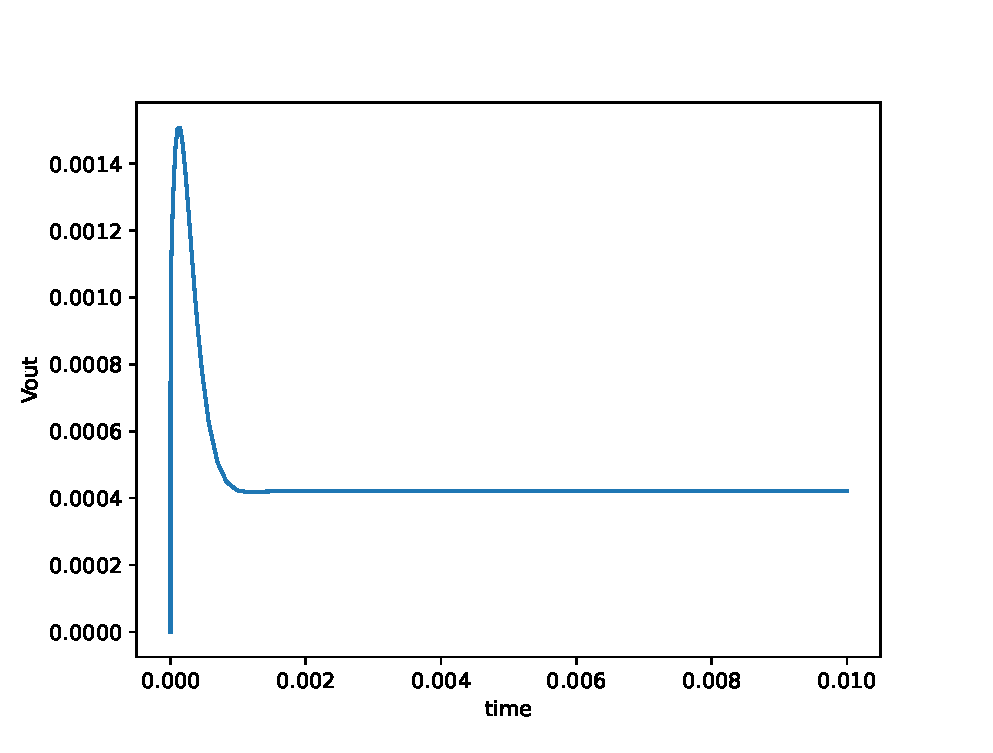
\includegraphics[width=\columnwidth]{./figs/ee18btech11049/ee18btech11049_1.eps}
\caption{Simulation result}
\label{fig:ee18btech11049_original}
\end{figure}

%%%%%%%%%%%%%%%%%%%%%%%%%%%%%%%%%%%%%%%%%%%%%%%%%%%%%%%%%%%%%%5
\item spice simulation after changing capacitance to 1.6nF 
\begin{itemize}
\item Refer to Fig. \ref{fig:ee18btech11049_original}
 for the spice output, $f_r = 8.5 khz$  
\item original netlist simulated circuit here:
\begin{lstlisting}
codes/ee18btech11049/ee18btech11049_2.net
\end{lstlisting}
\item You can find the python script for the above, used to generate the output here:
\begin{lstlisting}
codes/ee18btech11049/ee18btech11049_2.py
\end{lstlisting}
\end{itemize}

\begin{figure}[!ht]
\centering
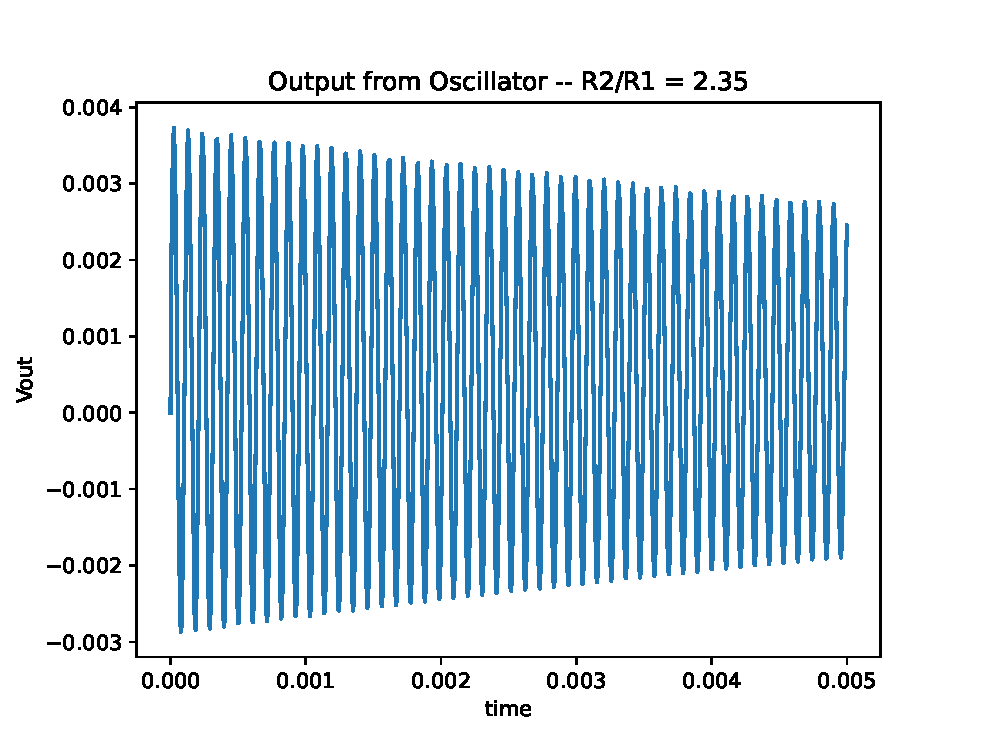
\includegraphics[width=\columnwidth]{./figs/ee18btech11049/ee18btech11049_2.eps}
\caption{Simulation result}
\label{fig:ee18btech11049_final}
\end{figure}


%%%%%%%%%%%%%%%%%%%%%%%%%%%%%%%%%%%%%%%%%%%%%%%%%%%%%%%%%%5

\item spice simulation after changing shunt resistance to restore frequency  
\begin{itemize}
\item Refer to Fig. \ref{fig:ee18btech11049_original}
 for the spice output, $f_r = 10 khz$  
\item original netlist simulated circuit here:
\begin{lstlisting}
codes/ee18btech11049/ee18btech11049_3.net
\end{lstlisting}
\item You can find the python script for the above, used to generate the output here:
\begin{lstlisting}
codes/ee18btech11049/ee18btech11049_3.py
\end{lstlisting}
\end{itemize}

\begin{figure}[!ht]
\centering
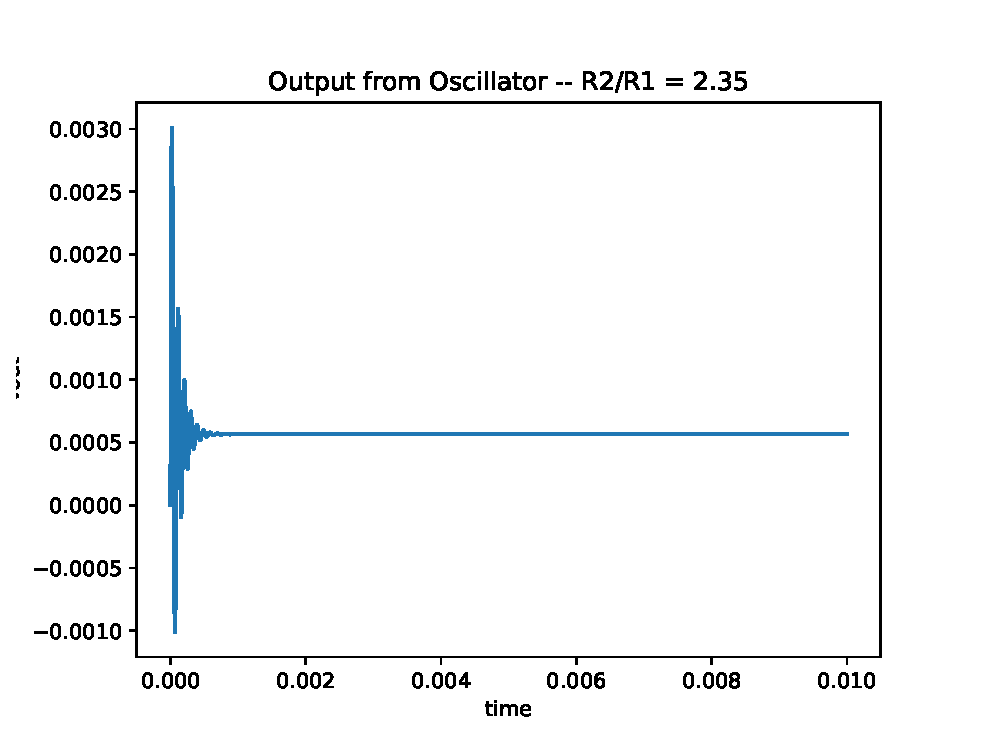
\includegraphics[width=\columnwidth]{./figs/ee18btech11049/ee18btech11049_3.eps}
\caption{Simulation result}
\label{fig:ee18btech11049_final}
\end{figure}

%%%%%%%%%%%%%%%%%%%%%%%%%%%%%%%%%%%%%%%%%%%%%%%%%%%%%%%%

\item spice simulation after changing $R_2/R_1$ to restore oscillations  
\begin{itemize}
\item Refer to Fig. \ref{fig:ee18btech11049_original}
 for the spice output, $f_r = 10 khz $  
\item original netlist simulated circuit here:
\begin{lstlisting}
codes/ee18btech11049/ee18btech11049_4.net
\end{lstlisting}
\item You can find the python script for the above, used to generate the output here:
\begin{lstlisting}
codes/ee18btech11049/ee18btech11049_4.py
\end{lstlisting}
\end{itemize}

\begin{figure}[!ht]
\centering
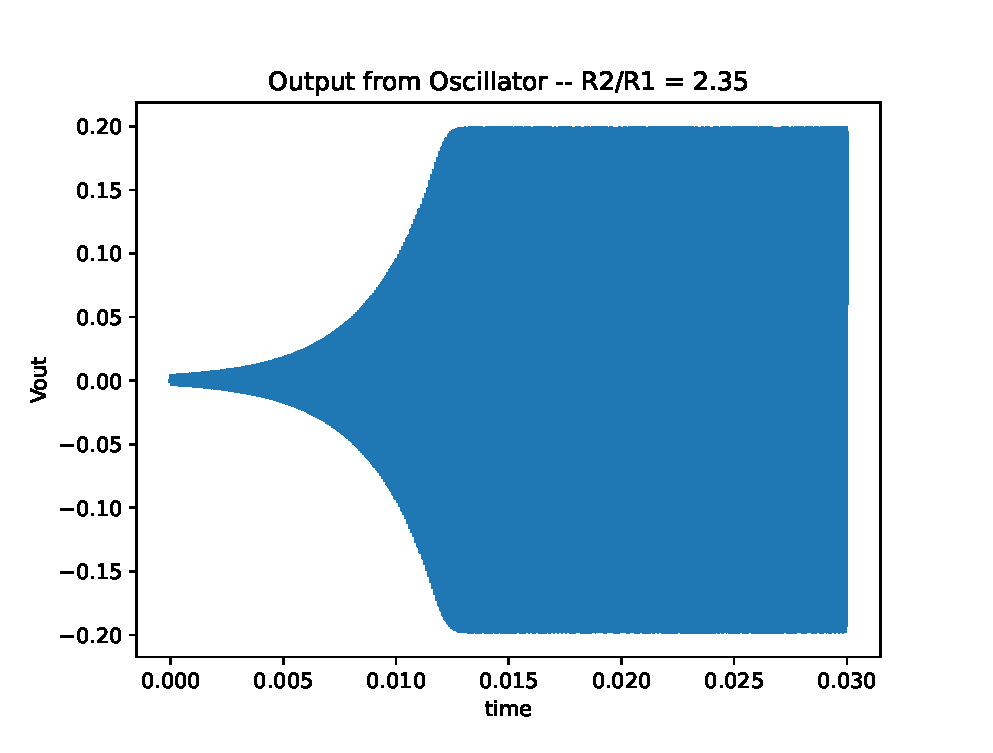
\includegraphics[width=\columnwidth]{./figs/ee18btech11049/ee18btech11049_4.eps}
\caption{Simulation result}
\label{fig:ee18btech11049_final}
\end{figure}

\end{enumerate}

\end{document}
